\documentclass[aspectratio=169]{beamer}
%
% Choose how your presentation looks.
%
% For more themes, color themes and font themes, see:
% http://deic.uab.es/~iblanes/beamer_gallery/index_by_theme.html
%
\mode<presentation>
{
  \usetheme{metropolis}      % or try Darmstadt, Madrid, Warsaw, ...
  \usecolortheme{metropolis-imagelab} % or try albatross, beaver, crane, ...
  \usefonttheme{structurebold}  % or try serif, structurebold, ...
  \setbeamercolor{background canvas}{bg=white}
  \setbeamertemplate{navigation symbols}{}
  \setbeamertemplate{bibliography item}{\insertbiblabel}
  %\setbeamertemplate{caption}[numbered]
} 
\usepackage[english]{babel}
\usepackage[utf8x]{inputenc}
\usepackage{algorithmic}
\usepackage{hyperref}
\usepackage{listings}             % Include the listings-package
\hypersetup{
    colorlinks = true,
    linkcolor = {mImagelabRed},
    urlcolor = {mImagelabRed}
}
\usepackage{animate}

\DeclareMathOperator*{\argmin}{arg\,min}

\title[Q-Learning]{Q-Learning}
\subtitle{Pattern Recognition and Machine Learning - 2017}
\institute{University of Modena and Reggio Emilia}
\author{Andrea Palazzi, Davide Abati}
\date{\today}

\def\thisframelogos{}

\newcommand{\framelogo}[1]{\def\thisframelogos{#1}}

\begin{document}

\framelogo{logo_unimore_white.png}

\bgroup
\renewcommand{\insertframenumber}{}
\begin{frame}[noframenumbering]
  \titlepage
\end{frame}
\egroup
\bgroup
\begin{frame}{Problem setting}
\begin{minipage}{0.5\textwidth}
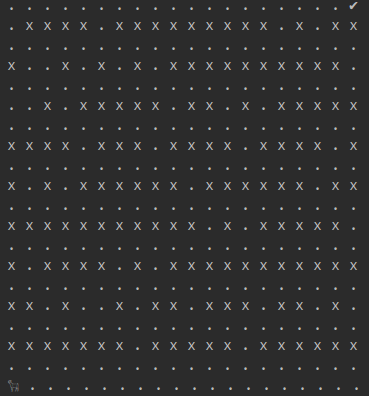
\includegraphics[width=0.9\textwidth]{img/env.png}
\end{minipage}
\begin{minipage}{0.45\textwidth}
We have an agent stuck in a maze.
\begin{itemize}
\item state is (x,y) position
\item reward is -1 for each time step
\item when the exit of the labirinth is reached, the episode terminates
\item allowed actions are N,S,W,E
\end{itemize}
Guide him out with reinforcement learning!
\end{minipage}
\end{frame}
\egroup
\bgroup
\begin{frame}{Q-learning algorithm for off-policy control}
\begin{algorithmic}
\STATE Initialize $Q(s,a), \forall s \in S, a \in \mathcal{A}(s)$, arbitrarily, and $Q(terminal-state, \dot)=0$
\FOR{each episode}
\STATE Intialise $S$
\FOR {each step of episode}
\STATE Choose $A$ from $S$ using policy derived from $Q$ (e.g., $\epsilon$-greedy)
\STATE Take action $A$, observe $R$, $S^{\prime}$
\STATE $Q(S,A) \leftarrow Q(S,A) + \alpha (R + \gamma \max_{a}(Q(S^{\prime}, a) - Q(S,A))$
\STATE $S \leftarrow S^{\prime}$
\ENDFOR
\ENDFOR
\end{algorithmic}
\end{frame}
\egroup
\bgroup
\begin{frame}{SARSA algorithm for on-policy control}
\begin{algorithmic}
\STATE Initialize $Q(s,a), \forall s \in S, a \in \mathcal{A}(s)$, arbitrarily, and $Q(terminal-state, \dot)=0$
\FOR{each episode}
\STATE Intialise $S$
\STATE Choose $A$ from $S$ using policy derived from $Q$ (e.g., $\epsilon$-greedy)
\FOR {each step of episode}
\STATE Take action $A$, observe $R$, $S^{\prime}$
\STATE Choose $A^{\prime}$ from $S^{\prime}$ using policy derived from $Q$ (e.g., $\epsilon$-greedy)
\STATE $Q(S,A) \leftarrow Q(S,A) + \alpha (R + \gamma (Q(S^{\prime}, A^{\prime}) - Q(S,A))$
\STATE $S \leftarrow S^{\prime}; A \leftarrow A^{\prime}$
\ENDFOR
\ENDFOR
\end{algorithmic}
\end{frame}
\egroup
\bgroup
\begin{frame}{More fun with gym!}
If you are curious about RL, try \href{https://github.com/openai/gym}{gym}:
\begin{center}
pip install gym
\end{center}
\centering
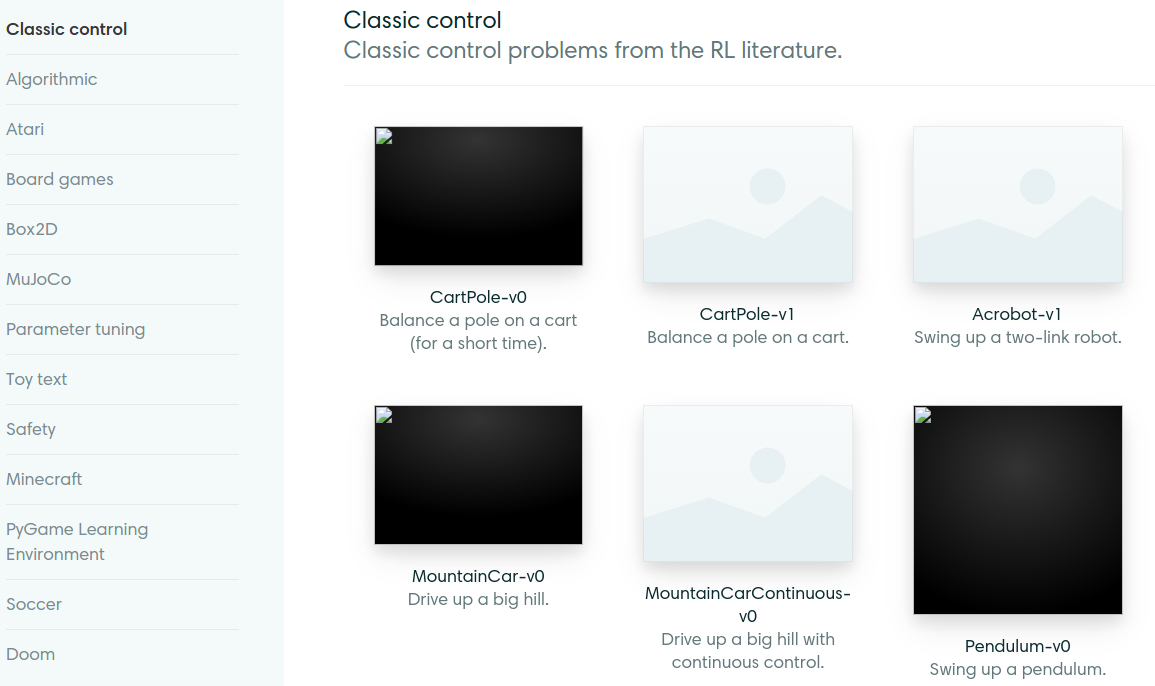
\includegraphics[width=0.5\textwidth]{img/gym.png}
\end{frame}
\egroup

\end{document}